% !TEX encoding = UTF-8 Unicode
\documentclass[a4paper]{article}

\usepackage{color}
\usepackage{url}
\usepackage[T2A]{fontenc} % enable Cyrillic fonts
\usepackage[utf8]{inputenc} % make weird characters work
\usepackage{graphicx}
\usepackage{listings}
\usepackage{multicol}
\usepackage{geometry}
\usepackage{lipsum}

%\usepackage[nottoc]{tocbibind}

\usepackage[english,serbian]{babel}
%\usepackage[english,serbianc]{babel} %ukljuciti babel sa ovim opcijama, umesto gornjim, ukoliko se koristi cirilica

\usepackage[unicode]{hyperref}
\hypersetup{colorlinks,citecolor=green,filecolor=green,linkcolor=blue,urlcolor=blue}

%\newtheorem{primer}{Пример}[section] %ćirilični primer
\newtheorem{primer}{Primer}[section]

\definecolor{mygreen}{rgb}{0,0.6,0}
\definecolor{mygray}{rgb}{0.5,0.5,0.5}
\definecolor{mymauve}{rgb}{0.58,0,0.82}
\definecolor{greyish}{rgb}{0.97,0.97,0.97}


\lstset{ 
  backgroundcolor=\color{greyish},   % choose the background color; you must add \usepackage{color} or \usepackage{xcolor}; should come as last argument
  basicstyle=\scriptsize\ttfamily,        % the size of the fonts that are used for the code
  breakatwhitespace=false,         % sets if automatic breaks should only happen at whitespace
  breaklines=true,                 % sets automatic line breaking
  captionpos=b,                    % sets the caption-position to bottom
  commentstyle=\color{mygreen},    % comment style
  deletekeywords={...},            % if you want to delete keywords from the given language
  escapeinside={\%*}{*)},          % if you want to add LaTeX within your code
  extendedchars=true,              % lets you use non-ASCII characters; for 8-bits encodings only, does not work with UTF-8
  firstnumber=1,                   % start line enumeration with line 1000
  frame=single,	                   % adds a frame around the code
  keepspaces=true,                 % keeps spaces in text, useful for keeping indentation of code (possibly needs columns=flexible)
  keywordstyle=\color{blue},       % keyword style
  language=Python,                 % the language of the code
  morekeywords={*,...},            % if you want to add more keywords to the set
  numbers=left,                    % where to put the line-numbers; possible values are (none, left, right)
  numbersep=5pt,                   % how far the line-numbers are from the code
  numberstyle=\tiny\color{mygray}, % the style that is used for the line-numbers
  rulecolor=\color{black},         % if not set, the frame-color may be changed on line-breaks within not-black text (e.g. comments (green here))
  showspaces=false,                % show spaces everywhere adding particular underscores; it overrides 'showstringspaces'
  showstringspaces=false,          % underline spaces within strings only
  showtabs=false,                  % show tabs within strings adding particular underscores
  stepnumber=2,                    % the step between two line-numbers. If it's 1, each line will be numbered
  stringstyle=\color{mymauve},     % string literal style
  tabsize=2,	                   % sets default tabsize to 2 spaces
  title=\lstname                   % show the filename of files included with \lstinputlisting; also try caption instead of title
}

\definecolor{dkgreen}{rgb}{0,0.6,0}
\definecolor{gray}{rgb}{0.5,0.5,0.5}
\definecolor{mauve}{rgb}{0.58,0,0.82}


\begin{document}

\title{\textbf{Predviđanje filmskih rejtinga}\\
\small{Projekat u okviru kursa Mašinsko učenje}}

\author{Nenad Perišić\\perisicnenad96@gmail.com\\}

\medskip

\newpage

\maketitle

%\begin{figure}[hb!]
%\begin{center}
%\small{Matematički fakultet \\ u Beogradu\\}
%
\includegraphics[scale=0.5]{matf_logo.png}
%\end{center}
%\end{figure}

%\vfill
\vspace{2cm}
\begin{figure}[b!]
\begin{center}

\includegraphics[scale=0.67]{matf_logo.png} \\
\small{Matematički fakultet \\ u Beogradu}
\end{center}
\end{figure}


\pagebreak

\tableofcontents

\newpage

\section{Uvod}
\label{sec:uvod}

U ovom radu ću pokušati da dam odgovor na pitanje da li je moguće predvideti rejting filma i proceniti njegovu uspešnost pre nego što on bude pušten u bioskopima. Ovo ću uraditi analiziranjem skupova multimodalnih podataka sa raznim atributima (svojstvima) kao što su režiser tog filma, glumačka ekipa, produkcijska kuća, opis filma, žanr filma, poster filma, budžet, vreme trajanja filma itd. Fokus će biti predviđanje rejtinga na osnovu tekstualnih atributa i primene algoritama linearne regresije, grebene regresije, slučajnih šuma na njima.


\section{Skup podataka}
\label{sec:skupPodataka}

Koriste se dva skupa podataka, "The movie dataset" \cite{movieDataset} i "Movie genre from its poster dataset" \cite{movieGenres}, oba dostupni na Kaggle \cite{kaggle} veb sajtu. Oni sadrže metapodatke za 45000 filmova koji su objavljeni pre jula 2017. godine. Podaci se sastoje od glumačke ekipe (cast), celokupne ekipe (crew), ključnih reči radnje, budžeta, prihoda, postera, datuma objavljivanja, jezika, produkcijskih kuća, država, broja glasova i njihovog proseka.\\

Skup podataka je organizovan na sledeći način:
\begin{itemize}
	\item \textit{movies\_metadata.csv} - glavna datoteka metapodataka o filmovima
	\item \textit{keywords.csv} - sadrži ključne reči filmskog zapleta dostupog u formi JSON objekta
	\item \textit{credits.csv} - sastoji se od glumačke ekipe takođe u formi JSON objekta
	\item \textit{links.csv} - sadrži TMDB i IMDB id-ove svih filmova
	\item \textit{ratings\_small.csv} - sadrži rejtinge od 100 000 rejtinga koji su prikupljeni od 700 korisnika na 9000 filmova
	\item \textit{movie\_genre.csv} - sadrži žanrove filmova koje ćemo spajati preko imdb\_id-a, a koja takođe sadrži i link do postera filma
\end{itemize}


\section{Preprocesiranje}
\label{sec:preprocesiranje}

Nakon spajanja svih navedenih tabela, uklonićemo kolone koje se ponavljaju, a to su: \textit{Title}, \textit{Original title}. Zatim uklanjamo još i kolone \textit{Poster} - link do postera filma, \textit{homepage} - link do stranice filma, \textit{belongs\_to\_collection}.\\

Za ulazne parametre posmatraćemo atribute cast, crew, synopses, genre i runtime, a IMDB Score ćemo uzeti za cilj predvidjanja. Iz kolona cast i crew ćemo da izdvojimo dva glavna glumca, režisera i prve dve produkcijske kuće za svaki film ali tako da su se pojavljivali u barem 5 filmova kako nam se ne bi narušilo predviđanje ukoliko je neko imao samo jedan film u svojoj karijeri. Takođe, zarad boljih rezultata možemo uzeti samo filmove koji su prvi put prikazani posle 1970. godine i čiji je originalni jezik engleski.\\

Nakon izdvajanja potrebnih atributa iz JSON formata uradićemo binarizaciju nad atributima \textit{Genre}, \textit{actors} i \textit{companies} koje smo izdvojili.
Što se tiče kolone \textit{overview} (synopses) koristićemo biblioteku \textit{spacy} \cite{spacy} za tokenizaciju i ostavićemo samo reči koje se javljaju u bar 20 filmova.\\

Podela podataka na trening i test skup je izvršena u odnosu 70\%:30\%.\\

\section{Vizuelizacija podataka}
\label{sec:vizuelizacija}

U ovoj sekciji će na grafički način biti prikazana zavisnost budžeta, vremena trajanja filma i raznih žanrova od rejtinga filma. Vizuelizacija je urađena nakon preprocesiranja i izdvajanja određenih atributa iz JSON formata. Na slici \ref{fig:horror} se može videti da filmovi čiji je žanr \textit{horror} imaju nešto manji rejting od onih koji imaju drugi žanr. Na slici  \ref{fig:documentary} možemo videti da filmovi čiji je žanr \textit{documentary} u znatno većem broju imaju viši rejting. Dakle kolonu \textit{genre} treba uzeti u razmatranje prilikom treniranja modela.


\begin{figure}[h!]
\centering
\begin{minipage}{.5\textwidth}
  \centering
  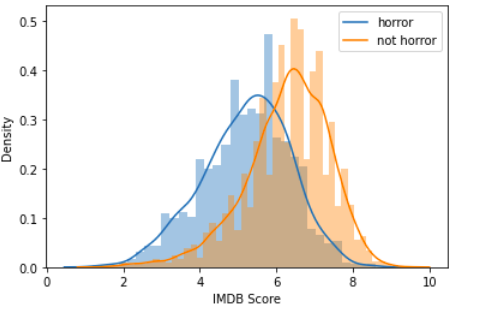
\includegraphics[scale=0.4]{horror.png}
  \caption{Genre: Horror}{}
  \label{fig:horror}
\end{minipage}%
\begin{minipage}{.5\textwidth}
  \centering
%  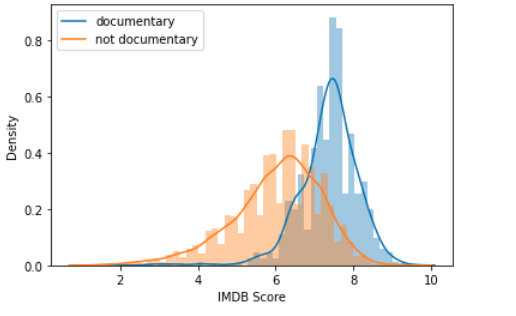
\includegraphics[width=.8\linewidth]{documentary.png}
  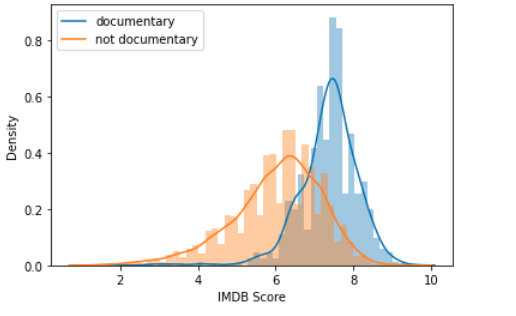
\includegraphics[scale=0.4]{documentary.png}
   \caption{Genre: documentary}{}
  \label{fig:documentary}
\end{minipage}
\end{figure}

Pokušajmo sada isto sa budžetom. Na slici \ref{fig:budget} se može zaključiti da ima nešto više filmova koji imaju budžet preko 5 miliona dolara, ali da njihov rejting nije nužno viši u odnosu na filmove sa manjim budžetom.

\begin{figure}[h!]
\begin{center}
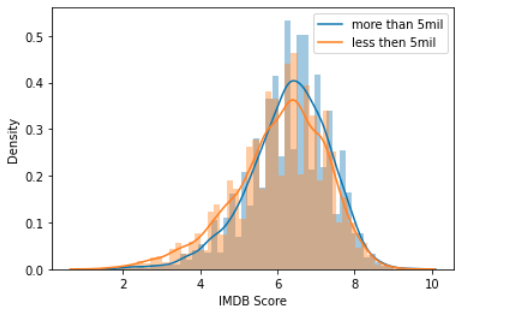
\includegraphics[scale=0.5]{budget.png}
\caption{Budget}
\label{fig:budget}
\end{center}
\end{figure}

Na kraju možemo da pogledamo još i dužinu trajanja filma u odnosu na rejting. Na slici \ref{fig:runtime} možemo videti da filmovi koji traju duže od 2 sata imaju bolji rejting u odnosu na one čija je dužina kraća od 2 sata pa ćemo i tu kolonu kasnije uzeti u razmatranje za treniranje modela.
\begin{figure}[h!]
\begin{center}
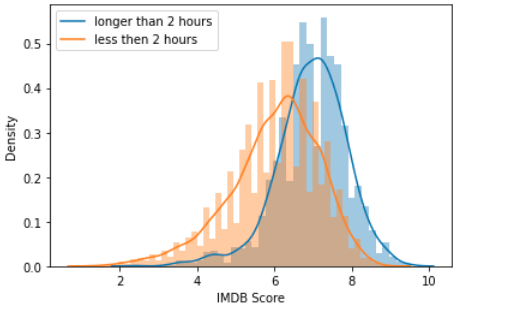
\includegraphics[scale=0.5]{runtime.png}
\caption{Runtime}
\label{fig:runtime}
\end{center}
\end{figure}


\section{Modeli}
\label{sec:modeli}

U ovoj sekciji ćemo kreirati regresione modele nad preprocesiranim podacima i evaluirati pomoću kvadratne greške (\textbf{${R}^2$}), srednje apsolutne (\textbf{MAE}) i srednje kvadratne greške (\textbf{MSE}).
Modeli koji ce biti trenirani nad podacima su:
\begin{itemize}
	\item Linear Regression
	\item Ridge Regression
	\item Lasso Regression
	\item Random Forest Regression
	\item Extreme Gradient Boosting
\end{itemize}

Kao što smo mogli da vidimo na graficima bitni atributi koji će biti od značaja za treniranje modela su: \textit{Genre, actors, director, companies, overview}, a ciljna promenljiva je \textit{IMDB Score}. Nakon završenog preprocesiranja i podele skupa na trening i test možemo da krenemo sa treniranjem modela nad tim podacima.



\subsection{Linearna regresija}
\label{sec:linearna_1}

Rezultati linearne regresije na trening i test skupu sa \textit{default} parametrima se mogu videti u tabeli \ref{table:table_1}.

\begin{table}[h!]
\caption{Errors}
\centering % used for centering table
\begin{tabular}{c c c c} % centered columns (4 columns)
\hline\hline %inserts double horizontal lines
 & ${R}^2$ & MAE & MSE \\ [0.2ex] % inserts table
%heading
\hline % inserts single horizontal line
train & 0.5469532634174328 & 0.6031675024259086 & 0.6228400675303715 \\ % inserting body of the table
test & 0.3615194589066031 & 0.7248295216204385 & 0.874435134094227 \\ [1ex] % [1ex] adds vertical space
\end{tabular}
\label{table:table_1}
\end{table}

Pošto rezultati nisu savršeni, isprobaćemo više modela sa različitim parametrima da vidimo kako se menjaju vrednosti grešaka modela. da bismo dobili što bolje rezultate. Ovo ćemo uraditi korišćenjem GridSearchCV metoda\cite{gridSearchCV}. Parametri koji su korišćeni su \textit{fit\_intercept: True, False, normalize: True, False}, \textit{scoring=r2} i za parametar cv je uzeta vrednost 5. Dobijene vrednosti su: \textit{best\_params: {fit\_intercept: True, 'normalize': False}}. Kada ponovo treniramo model sa novim parametrima, rezultati koje dobijamo se mogu videti u tabeli \ref{table:table_2}.

\begin{table}[h!]
\caption{Errors}
\centering % used for centering table
\begin{tabular}{c c c c} % centered columns (4 columns)
\hline\hline %inserts double horizontal lines
 & ${R}^2$ & MAE & MSE \\ [0.2ex] % inserts table
%heading
\hline % inserts single horizontal line
train & 0.5469532634174328 & 0.6031675024259086 & 0.6228400675303715 \\ % inserting body of the table
test & 0.3615194589066031 & 0.7248295216204385 & 0.874435134094227 \\ [1ex] % [1ex] adds vertical space
\end{tabular}
\label{table:table_2}
\end{table}

Dakle, može se zaključiti da su rezultati isti kao sa modelom koji je treniran sa \textit{default} parametrima.


\subsection{Grebena regresija}
\label{sec:ridge_1}

Rezultati grebene regresije na trening i test skupu sa parametrima \textit{alpha=10, normalize=True} se mogu videti u tabeli \ref{table:table_3}.

\begin{table}[h!]
\caption{Errors}
\centering % used for centering table
\begin{tabular}{c c c c} % centered columns (4 columns)
\hline\hline %inserts double horizontal lines
 & ${R}^2$ & MAE & MSE \\ [0.2ex] % inserts table
%heading
\hline % inserts single horizontal line
train & 0.14921849413953459 & 0.8430023954492178 & 1.169638290656023 \\ % inserting body of the table
test & 0.12596594545080564 & 0.8545487903574828 & 1.197038964388495 \\ [1ex] % [1ex] adds vertical space
\end{tabular}
\label{table:table_3}
\end{table}

Rezultati nisu dobri, greške odstupaju puno od svojih idealnih vrednosti, zbog toga probajmo sada GridSearchCV metod. Uzećemo sledeće vrednosti parametara: \textit{'alpha':[1,5,10,30], 'fit\_intercept':[True,False], 'normalize':[True,False]} i pustiti algoritam da radi. Najbolje dobijene vrednosti su: \textit{{'alpha': 1, 'fit\_intercept': True, 'normalize': True}}. Kada ponovo treniramo model sa novim parametrima, rezultati koje dobijamo se mogu videti u tabeli \ref{table:table_4}.

\begin{table}[h!]
\caption{Errors}
\centering % used for centering table
\begin{tabular}{c c c c} % centered columns (4 columns)
\hline\hline %inserts double horizontal lines
 & ${R}^2$ & MAE & MSE \\ [0.2ex] % inserts table
%heading
\hline % inserts single horizontal line
train & 0.4471618617605746 & 0.6677622829582377 & 0.7600313953296844 \\ % inserting body of the table
test & 0.35788726526000325 & 0.7228114470349141 & 0.879409628278469 \\ [1ex] % [1ex] adds vertical space
\end{tabular}
\label{table:table_4}
\end{table}

Vidimo da su rezultati dosta bolji sa parametrima koje je GridSearchCV pronašao, ali i dalje nedovoljno dobro. Nastavimo dalje.


\subsection{Lasso regresija}
\label{sec:lasso_1}

Rezultati grebene regresije na trening i test skupu sa parametrom \textit{alpha=0.01} se mogu videti u tabeli \ref{table:table_5}.

\begin{table}[h!]
\caption{Errors}
\centering % used for centering table
\begin{tabular}{c c c c} % centered columns (4 columns)
\hline\hline %inserts double horizontal lines
 & ${R}^2$ & MAE & MSE \\ [0.2ex] % inserts table
%heading
\hline % inserts single horizontal line
train & 0.3067452704795627 & 0.7552564534961796 & 0.9530734639152751 \\ % inserting body of the table
test & 0.304028552361731 & 0.752210485497123 & 0.953172175144332 \\ [1ex] % [1ex] adds vertical space
\end{tabular}
\label{table:table_5}
\end{table}

Sa GridSearchCV metodom za parametara: \textit{'alpha':[0.1, 0.01, 0.5], 'fit\_interceptTrue,False], 'normalize':[True,False], 'selection':['cyclic', 'random']} se ne dobija nikakvo poboljšanje.



\subsection{Slučajne šume}
\label{sec:randomForest_1}

Probajmo sa slučajnim šumama da li možemo da dobijemo bolje rezultate od dosadašnjih. Pokrenućemo algoritam za dubinu 32. Na osnovu rezultata u tabeli \ref{table:table_6} zaključujemo da je algoritam slučajnih šuma do sada doe najbolje rezultate.

\begin{table}[h!]
\caption{Errors}
\centering % used for centering table
\begin{tabular}{c c c c} % centered columns (4 columns)
\hline\hline %inserts double horizontal lines
 & ${R}^2$ & MAE & MSE \\ [0.2ex] % inserts table
%heading
\hline % inserts single horizontal line
train & 0.7741702821868292 & 0.4291284543398816 & 0.3104664162336058 \\ % inserting body of the table
test & 0.3865944458760707 & 0.6995345386544246 & 0.8400935243162557 \\ [1ex] % [1ex] adds vertical space
\end{tabular}
\label{table:table_6}
\end{table}

Nakon provere najboljih parametara sa GridSearchCV metodom, dobijeni rezultati su se neznatno poboljšali kao što se može videti u tabeli \ref{table:table_7}.

\begin{table}[h!]
\caption{Errors}
\centering % used for centering table
\begin{tabular}{c c c c} % centered columns (4 columns)
\hline\hline %inserts double horizontal lines
 & ${R}^2$ & MAE & MSE \\ [0.2ex] % inserts table
%heading
\hline % inserts single horizontal line
train & 0.5893342000209669 & 0.5757413356809938 & 0.5645755590709117 \\ % inserting body of the table
test & 0.4007266263235302 & 0.6939344630588781 & 0.8207387056346158 \\ [1ex] % [1ex] adds vertical space
\end{tabular}
\label{table:table_7}
\end{table}

\subsection{Extreme gradient boosting}
\label{sec:xgBoost_1}

Na kraju, probaćemo još i \textit{gradient boosting} algoritam. Dobijeni rezultati u tabeli \ref{table:table_8} su najbolji od svih modela koje smo do sada probali.

\begin{table}[h!]
\caption{Errors}
\centering % used for centering table
\begin{tabular}{c c c c} % centered columns (4 columns)
\hline\hline %inserts double horizontal lines
 & ${R}^2$ & MAE & MSE \\ [0.2ex] % inserts table
%heading
\hline % inserts single horizontal line
train & 0.5674401301819887 & 0.5913678678131937 & 0.5946751113596823 \\ % inserting body of the table
test & 0.4355463606452872 & 0.6716326508373056 & 0.7730511144064957 \\ [1ex] % [1ex] adds vertical space
\end{tabular}
\label{table:table_8}
\end{table}

Kada smo već kod ovog algoritma, možemo napraviti grafik bitnosti atributa za predikciju rejtinga. Na slici \ref{fig:featureImportance} se može videti da dužina filma, i žanr igraju veliku ulogu u oceni tog filma.

\begin{figure}[h!]
\begin{center}
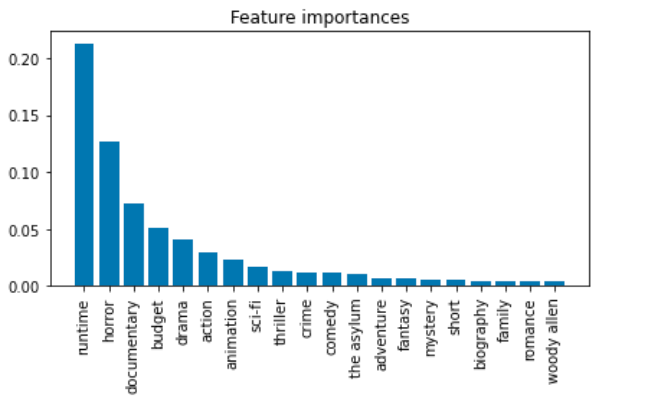
\includegraphics[scale=0.4]{featureImportance.png}
\caption{Feature importance}
\label{fig:featureImportance}
\end{center}
\end{figure}

\pagebreak

\subsection{Vizuelno poređenje modela}
\label{sec:plotting_1}

Sada ćemo vizuelno uporediti dobijene rezultate od svih modela, za svaku grešku posebno.

\begin{figure}[h!]
\begin{center}
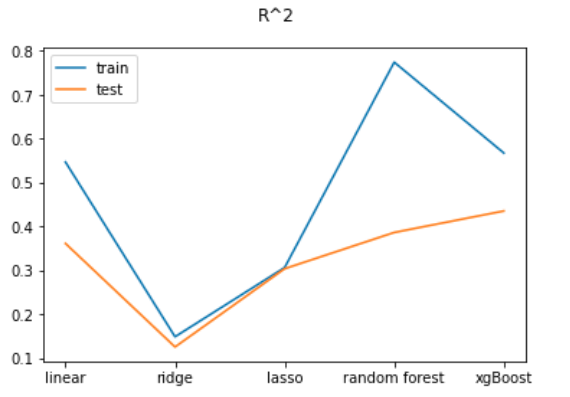
\includegraphics[scale=0.36]{r2.png}
\caption{MAE errors}
\label{fig:runtime}
\end{center}
\end{figure}

\begin{figure}[h!]
\begin{center}
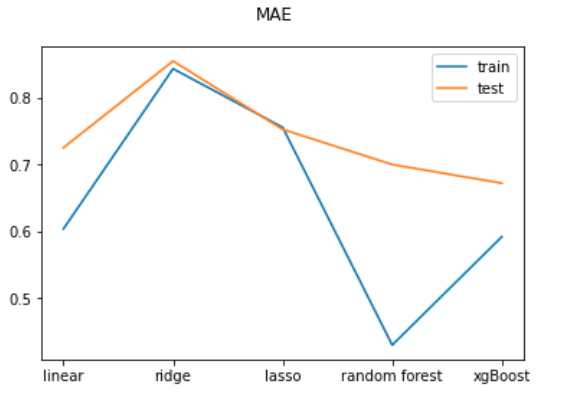
\includegraphics[scale=0.36]{mae.png}
\caption{MAE errors}
\label{fig:runtime}
\end{center}
\end{figure}

\begin{figure}[h!]
\begin{center}
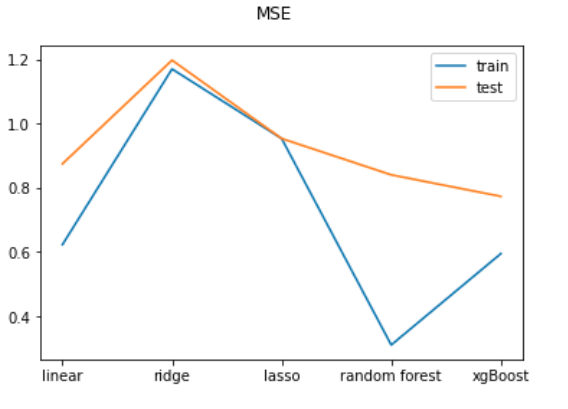
\includegraphics[scale=0.36]{mse.png}
\caption{MSE errors}
\label{fig:mse}
\end{center}
\end{figure}

Vidimo da xgBoost daje najbolje rezultate, a da ridge i lasso regresije najbolje generalizuju podatke.

%\pagebreak

\section{Ponovno preprocesiranje podataka}
\label{sec:preprocesiranje_2}

U cilju dobijanja koeficijenta determinacije što bliže vrednosti 1, a srednje absolutne i srednje kvadratne greske što bliže 0, pokušaćemo dodatno da obradimo ulazne podatke i da vidimo da li ćemo u tom slučaju dobiti bolje rezultate. Ideje za unapređenje su sledeće:

\begin{itemize}
	\item iz svakog filma ćemo uzeti pvih 6 glumaca, potom od njih izdvojiti 200 najfrekventnijih glumaca - onih koji se javljaju u najvećem broju filmova, izbaciti filmove gde oni ne glume, a potom primeniti binarizaciju
	\item da se poboljša tokenizacija opisa filmova (\textit{synopses}) tako što ćemo koristeći nltk biblioteku izbaciti stop reči, jako učestale reči i specijalne karaktere kako bismo smanjili broj kolona u podacima na kojima ćemo trenirati modele
	\item standardizacija atributa \textit{runtime} i \textit{budget}
\end{itemize}


\section{Modeli sa poboljšanim preprocesiranjem}
\label{sec:modeli_2}

Nakon izvršenog ponovnog preprocesiranja, može se primetiti da se broj atributa značajno smanjio, sa 4993 na 1959. Istrenirajmo sada ponovo modele i pogledajmo da li će rezultati biti bolji ili ne.

\subsection{Linearna regresija}
\label{sec:linearna_regresija_2}

Dobijeni rezultati linearne regresije se mogu videti u tabeli \ref{table:table_9}.

\begin{table}[h!]
\caption{Errors}
\centering % used for centering table
\begin{tabular}{c c c c} % centered columns (4 columns)
\hline\hline %inserts double horizontal lines
 & ${R}^2$ & MAE & MSE \\ [0.2ex] % inserts table
%heading
\hline % inserts single horizontal line
train & 0.6975373878682696 & 0.4414965886950981 & 0.325694684152396 \\ % inserting body of the table
test & 0.08361906453769419 & 0.8171506801963895 & 1.0701402184640283 \\ [1ex] % [1ex] adds vertical space
\end{tabular}
\label{table:table_9}
\end{table}

Nakon puštanja GridSearchCV algoritma, nisu dobijeni ništa bolji rezultati.

\subsection{Grebena regresija}
\label{sec:grebena_regresija_2}

Rezultati grebene regresije se mogu videti u tabeli \ref{table:table_10}. Sa GridSearchCV metodom, rezultati su malo bolji (tabela \ref{table:table_11}).

\begin{table}[h!]
\caption{Errors}
\centering % used for centering table
\begin{tabular}{c c c c} % centered columns (4 columns)
\hline\hline %inserts double horizontal lines
 & ${R}^2$ & MAE & MSE \\ [0.2ex] % inserts table
%heading
\hline % inserts single horizontal line
train & 0.19174609984964475 & 0.7217692891909088 & 0.8703356651888018 \\ % inserting body of the table
test & 0.12165415806380964 & 0.7268126983311105 & 0.8674203342644023 \\ % [1ex] adds vertical space
\end{tabular}
\label{table:table_10}
\end{table}

\begin{table}[h!]
\caption{Errors}
\centering % used for centering table
\begin{tabular}{c c c c} % centered columns (4 columns)
\hline\hline %inserts double horizontal lines
 & ${R}^2$ & MAE & MSE \\ [0.2ex] % inserts table
%heading
\hline % inserts single horizontal line
train & 0.5430554470969404 & 0.5358217404979934 & 0.4920423413129251 \\ % inserting body of the table
test & 0.2672915613818133 & 0.6653916126978011 & 0.7235944754329561 \\  % [1ex] adds vertical space
\end{tabular}
\label{table:table_11}
\end{table}

\pagebreak

\subsection{Lasso regresija}
\label{sec:lasso_regresija_2}

Dobijeni rezultati lasso regresije se mogu videti u tabeli \ref{table:table_12}.

\begin{table}[h!]
\caption{Errors}
\centering % used for centering table
\begin{tabular}{c c c c} % centered columns (4 columns)
\hline\hline %inserts double horizontal lines
 & ${R}^2$ & MAE & MSE \\ [0.2ex] % inserts table
%heading
\hline % inserts single horizontal line
train & 0.22539566709947767 & 0.7071151600038588 & 0.8341014837140812 \\ % inserting body of the table
test & 0.23082228287647877 & 0.6769756376029746 & 0.7596101223924109 \\ [1ex] % [1ex] adds vertical space
\end{tabular}
\label{table:table_12}
\end{table}


\subsection{Slučajne šume}
\label{sec:slucajne_sume_2}

Dobijeni rezultati se mogu videti u tabeli \ref{table:table_13}.

\begin{table}[h!]
\caption{Errors}
\centering % used for centering table
\begin{tabular}{c c c c} % centered columns (4 columns)
\hline\hline %inserts double horizontal lines
 & ${R}^2$ & MAE & MSE \\ [0.2ex] % inserts table
%heading
\hline % inserts single horizontal line
train & 0.8434910739949135 & 0.3320578907345683 & 0.16853033458580594 \\ % inserting body of the table
test & 0.3480215435800472 & 0.6226180725231611 & 0.6438686717686649 \\ [1ex] % [1ex] adds vertical space
\end{tabular}
\label{table:table_13}
\end{table}

Slični rezultati su dobijeni i sa GridSearchCV metodom.

\subsection{Extreme gradient boosting}
\label{sec:xgBoost_2}

Dobijeni rezultati se mogu videti u tabeli \ref{table:table_14}.

\begin{table}[h!]
\caption{Errors}
\centering % used for centering table
\begin{tabular}{c c c c} % centered columns (4 columns)
\hline\hline %inserts double horizontal lines
 & ${R}^2$ & MAE & MSE \\ [0.2ex] % inserts table
%heading
\hline % inserts single horizontal line
train & 0.7356594644033094 & 0.40847821777075716 & 0.2846444611552286 \\ % inserting body of the table
test & 0.35436000629533615 & 0.6213208720406557 & 0.6376090514861819 \\ [1ex] % [1ex] adds vertical space
\end{tabular}
\label{table:table_14}
\end{table}

\pagebreak

\subsection{Vizuelno poređenje modela}
\label{sec:plotting_1}

Sada ćemo vizuelno uporediti dobijene rezultate od svih modela, za svaku grešku posebno.

\begin{figure}[h!]
\begin{center}
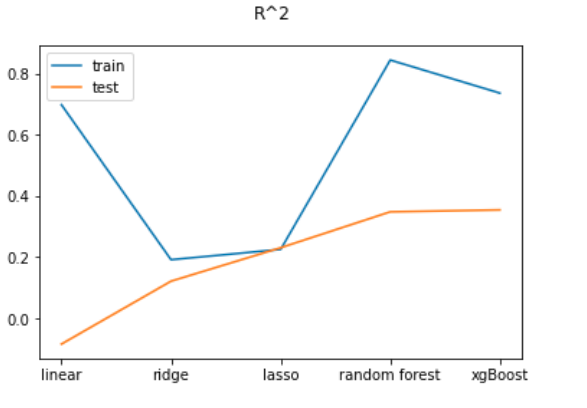
\includegraphics[scale=0.3]{r2_2.png}
\caption{${R}^2$ errors}
\label{fig:r2}
\end{center}
\end{figure}

\begin{figure}[h!]
\begin{center}
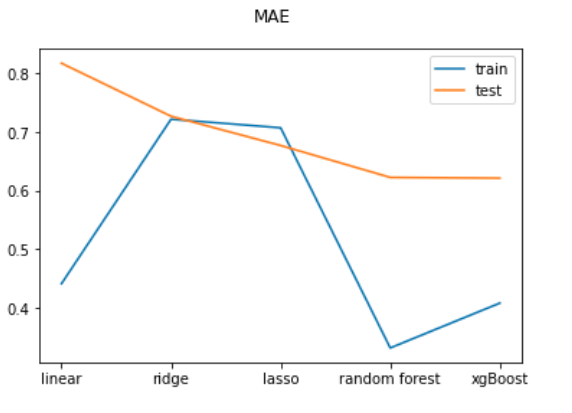
\includegraphics[scale=0.3]{mae_2.png}
\caption{MAE errors}
\label{fig:mae_2}
\end{center}
\end{figure}

\begin{figure}[h!]
\begin{center}
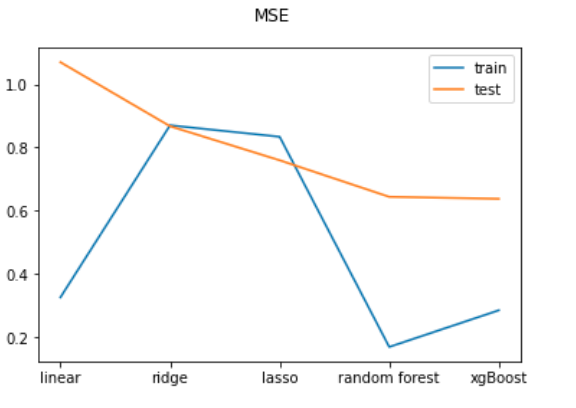
\includegraphics[scale=0.3]{mse_2.png}
\caption{MSE errors}
\label{fig:mse}
\end{center}
\end{figure}

Vidimo da xgBoost daje najbolje rezultate, a da ridge i lasso regresije najbolje generalizuju podatke.


\section{Zaključak}
\label{sec:zakljucak}

Isprobano je dosta modela nad različitim skupom podataka. Može se zaključiti da je najbolje rezultate dao model dobijen xgBoost regresijom, a da najbolju generalizaciju vrši lasso. Što se tiče atributa možemo da izvedemo zaključak da će zanr imati dosta uticaja na samu ocenu filma, na primer vidimo da ukoliko je film horor, dokumentarac, drama ili akcija će imati veću ocenu od ostalih. Dužina trajanja filma se takođe pokazala kao bitna stavka, dok se budžet pokazao kao manje bitan u odnosu na ova dva parametra.


\pagebreak

\addcontentsline{toc}{section}{Literatura}
\appendix
\bibliography{reference}
\bibliographystyle{ieeetr}
\appendix

\end{document}
